\section{Integración}

Inicialmente se planteó integración con la aplicación desarrollada en la primera práctica de la asignatura pero para esto serían necesarios servicios de pago de Google por lo que se desechó esta opción.

Al no poderse implementar en Android, se optó por crear un bot de telegram, simplemente generamos un bot de telegram y tomamos su token de acceso. Dentro de la sección de integraciones habilitamos Telegram e introducimos el token. Iniciamos nuestro bot con \texttt{/start} y ya es posible conversar con él.

Aunque existen otros métodos para interaccionar por voz, debido a falta de tiempo para el estudio e implementación de dichos métodos, en especial al no haberlos estudiado en clase, no hemos podido integrarlo en la aplicación. La única diferencia de usar el sistema de dialogo es que estas aplicaciones de integración detectarían la voz del usuario para reconocer los distintos intest de Dialogflow, y la respuesta la sintetizarían con una voz.

Algunas imágenes del sistema funcionando serían las siguientes:

\begin{figure}[H]
  \centering
      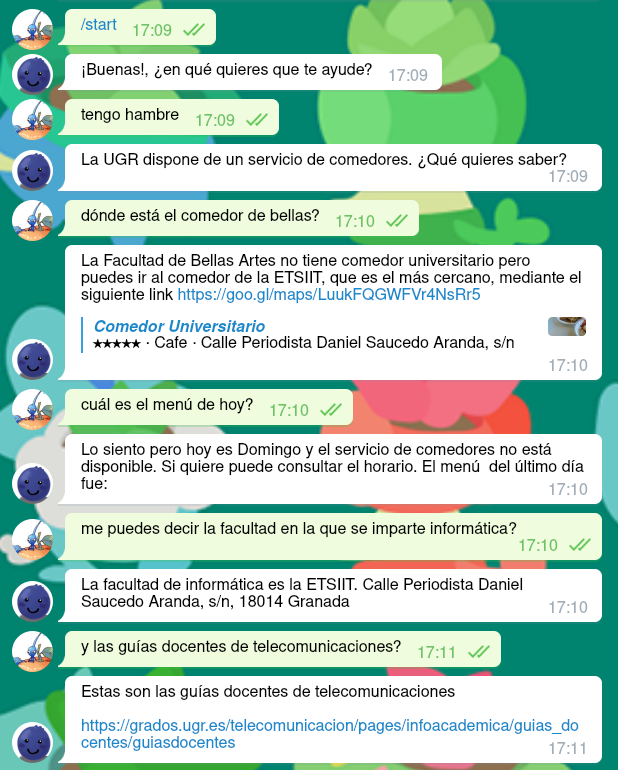
\includegraphics[width=\textwidth]{Aranbot.png}
 		\caption{Ejemplo de interacción con nuestro sistema de dialogo.}
\end{figure}


\begin{figure}[H]
  \centering
      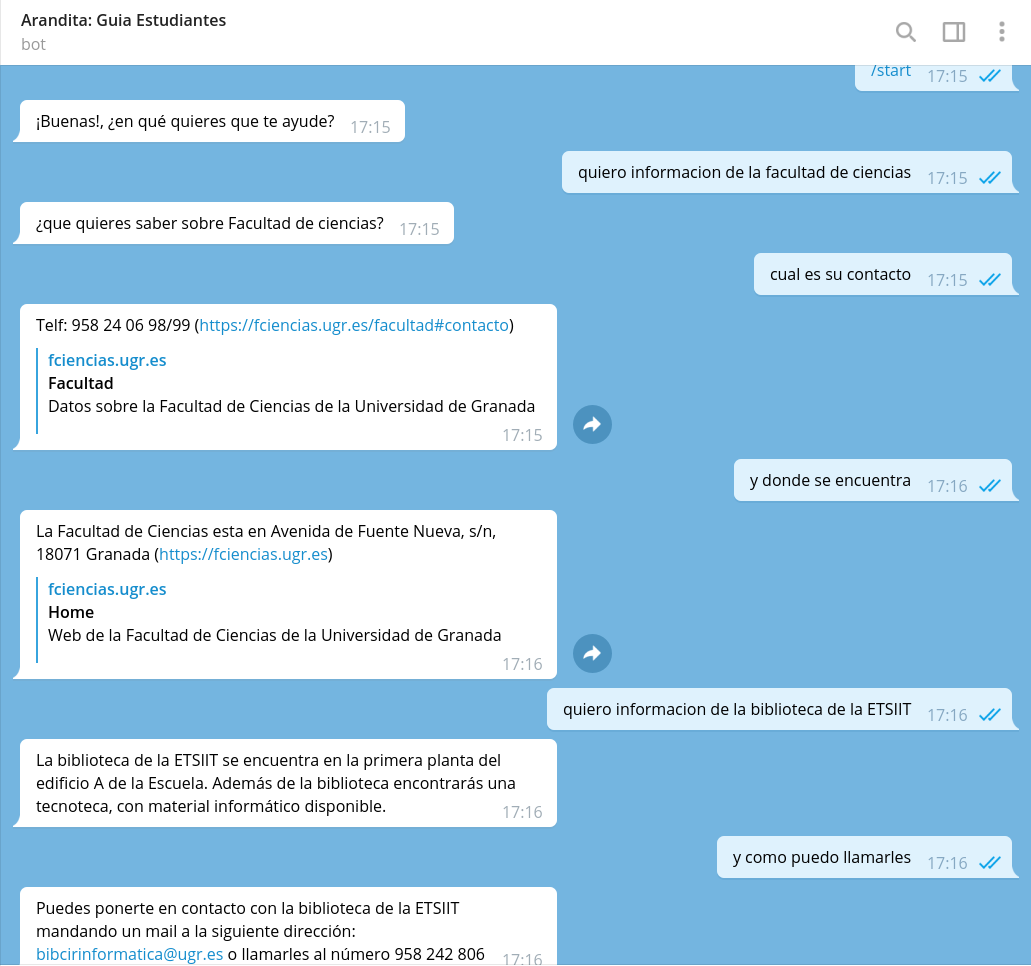
\includegraphics[width=\textwidth]{ej_conversacion.png}
 		\caption{Ejemplo de interacción con nuestro sistema de dialogo.}
\end{figure}

